\documentclass[polish,a4paper]{article}
% pakiet MwE
\usepackage{mwe}
% tytul referatu
\title{Tytuł referatu w języku polskim}
% tytul referatu w jez. angielskim
\titleEng{Tytuł referatu w języku angielskim}
% Autorzy
\author{
Imię Nazwisko\affmark[1], Imię Nazwisko\affmark[1], Imię Nazwisko\affmark[2]\\
\affaddr{\affmark[1] Afiliacja autorów 1 oraz 2}\\
\affaddr{\affmark[2] Afiliacja autora 3}
}

\begin{document}

\maketitle

Streszczenie referatu może obejmować maksymalnie dwie strony. Prosimy o przygotowanie streszczenia bez dokonywania podziału na rozdziały. Rozpocząć należy od podania tytułu wystąpienia – w języku polskim („Tytuł referatu w języku polskim”) i angielskim („Tytuł referatu w języku angielskim”), danych personalnych prelegenta („Imię i nazwisko prelegenta”) i afiliowanej jednostki naukowej („Afiliowana jednostka naukowa”).

Streszczenie referatu powinno być przygotowane za pomocą niniejszego szablonu. Pliki  *.tex oraz *.sty bądź *.docx wraz z zamieszczonymi w streszczeniach rysunkami (w formacie *.jpg lub *.png, każdy maksymalnie 1 MB) należy przesłać na adres \textbf{kme@pwr.edu.pl} do dnia \textbf{01.11.2020}.

W niniejszym przykładzie zamieszczono typowe, struktury (równania, tabele, rysunki, wyliczanie, literaturę) dokumentu LaTex. Należy je wypełnić swoją treścią.  Niepotrzebne, struktury można zawiesić stawiając na początku linii znak \% lub wymazać.

Rysunki wstawiamy w formacje *.jpg lub *.png w dobrej jakości (150dpi). Wszystkie wykożystane rysunki należy załączyć przy wysyłaniu streszczenia.

Pozycje literaturowe  podawać zgodnie ze wzorcem. Cytujemy używając np. $\backslash$cite\{Aref1\}  co utworzy \cite{Aref1}. Pierwszy raz kompilujemy dwukrotnie aby zostały wypełnione odwołania do literatury. W streszczeniu należy ograniczyć  liczbę cytowanych publikacji do najważniejszych 3.

Przykład \textbf{wyliczenia} (zamiast \textbf{itemize } można użyć \textbf{enumerate}, aby pozycje były numerowane).
\begin{itemize}
\item górny: 2,0 cm,
\item dolny: 2,0 cm
\item lewy:  3,5 cm
\item prawy: 2,0 cm
\end{itemize}

Przykład fragment tekstu z \textbf{równaniami} zamieszczono poniżej.
Równania ruchu lepkiego i nieściśliwego płynu mają postać (równanie \ref{eom} oraz \ref{incmp} - odniesienie do równania zapisujemy jako np. $\backslash$ref\{eom\}, natomiast równanie ma dodany $\backslash$label\{eom\}, który tworzy podstawę odniesienia) \cite{Kochin, Aref1}:
\begin{equation}\label{eom}
\frac{\partial{\mathbf{u}}}{\partial t}+(\mathbf{u} \cdot \nabla)\mathbf{u}=-\frac{1}{\rho}\nabla p+\nu \Delta \mathbf{u},
\end{equation}
\begin{equation}\label{incmp}
\nabla \cdot \mathbf{u}=0,
\end{equation}
gdzie $\mathbf{u}=(u,v,w)$ jest wektorem prędkości, $\rho$ -- gęstością płynu, $p$ -- ciśnieniem a $\nu$ -- kinematycznym współczynnikiem lepkości.

W dalszej części przedstawiono przykłady zamieszczania \textbf{wykresów, obrazków oraz tabel.}
Pojedynczy wykres lub zdjęcie (Rys. \ref{obraz1} - odniesienie do obrazu tworzymy analogicznie do przykładu z równaniem):
\begin{figure}[h!]
\centering
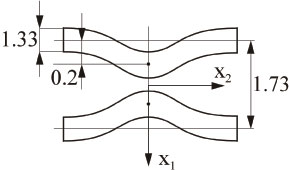
\includegraphics[width=0.35\linewidth]{figure1.jpg}
\caption{Jeden obrazek z podpisem}\label{obraz1}
\end{figure}

W celu zwiększenia czytelności zezwala się na wykorzystanie $\backslash$newpage
\newpage

Dwa wykresy lub zdjęcia obok siebie z dwoma niezależnymi popisami (Rys \ref{obraz2} oraz Rys. \ref{obraz3}):

\begin{figure}[htb]
\centering
\begin{minipage}[t]{0.42\linewidth}
\centering
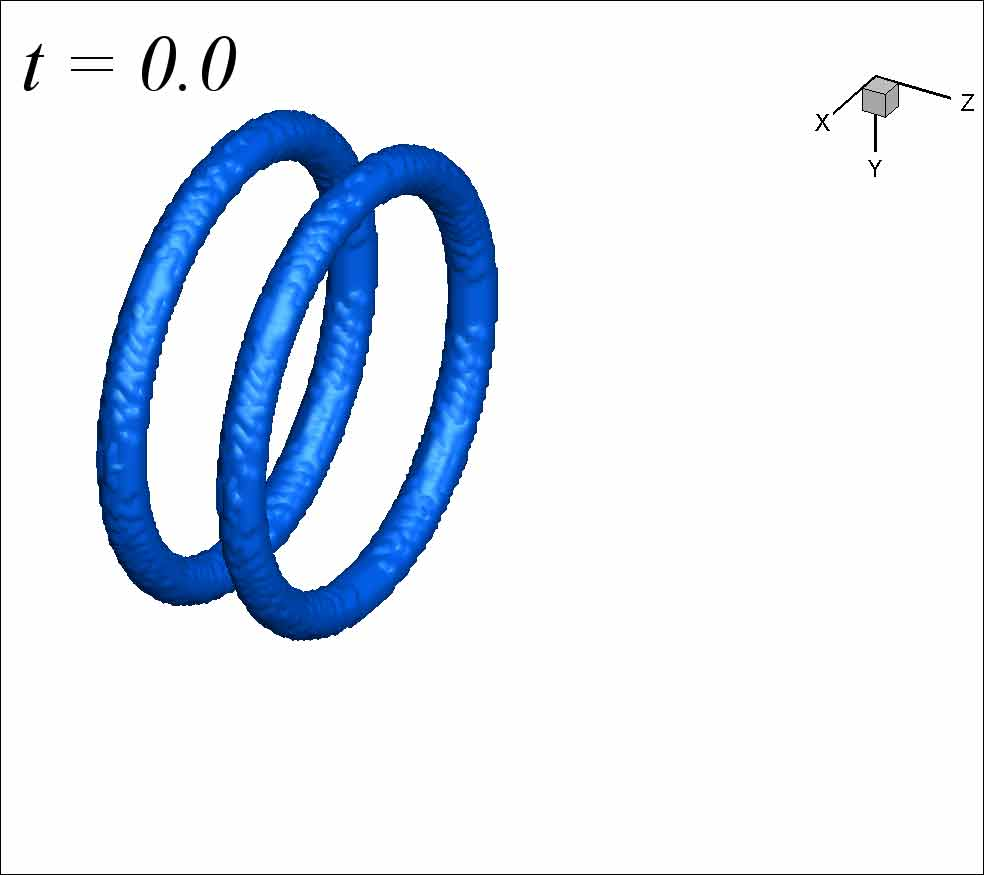
\includegraphics[width=0.65\linewidth]{figure1a.jpg}
\caption{Dwa obrazki obok siebie z dwoma podpisami (lewy)}\label{obraz2}
\end{minipage}
\quad
\begin{minipage}[t]{0.42\linewidth}
\centering
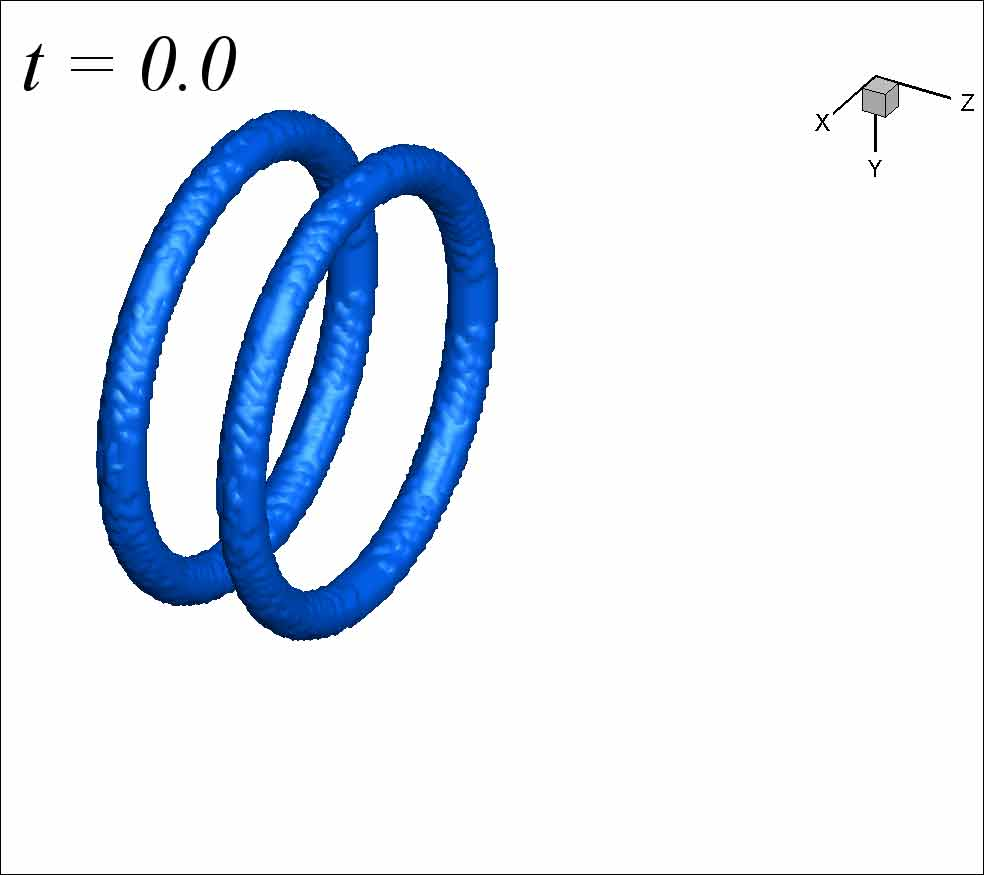
\includegraphics[width=0.65\linewidth]{figure1a.jpg}
\caption{Dwa obrazki obok siebie z dwoma podpisami (prawy)}\label{obraz3}
\end{minipage}
\end{figure}

Przykład tworzenia tabeli (Tab. \ref{tab1} oraz Tab. \ref{tab:cryocoolers}).\\
\begin{table} [!ht]
\caption{Przyspieszenie osiągane dla metody Jacobiego.}\label{tab1}
\centerline{
\begin{tabular}{|c|c|c|c|c|}
\hline
Liczba węzłów & tsl  &  tx &  nc & frm nc\\
\hline
32x32x32 & 4.05 & 6.61 & 6.94 & 12.32\\
64x64x64 & 17.71 & 26.32 & 31.26 & 52.82\\
128x128x128 & 24.78 & 29.95 & 43.67 & 58.89\\
\hline
\end{tabular}}
\end{table}

Dodatkowy przykład tworzenia tabeli.\\
\begin{table}[h]
    \centering
    \caption{Cryogenic coolers}
    \label{tab:cryocoolers}
    \begin{tabular}{@{}lll@{}}
    \toprule
    \begin{tabular}[c]{@{}c@{}}Cryooler\end{tabular} &
      \begin{tabular}[c]{@{}c@{}}Capacity range\end{tabular} &
      \multicolumn{1}{c}{ } \\ \midrule
    \begin{tabular}[c]{@{}c@{}}Turbo-Brayton\end{tabular}    & 18 - 250 kW at 120 K  \\
    \begin{tabular}[c]{@{}c@{}}Stirling\end{tabular}         & 2 - 8 kW at 120 K     \\
    \begin{tabular}[c]{@{}c@{}}Gifford-McMahon\end{tabular}  & 14 - 600 W at 80 K     \\
    \begin{tabular}[c]{@{}c@{}}2-stage Pulse Tube\end{tabular}  & up to 1.2 kW at 120 K  \\
    \begin{tabular}[c]{@{}c@{}}Single-stage Pulse Tube\end{tabular}  & 12 - 90 W at 80 K  \\
    \begin{tabular}[c]{@{}c@{}}Miniature Pulse Tube\end{tabular}       & 3 - 10 W at 80 K    \\
    \begin{tabular}[c]{@{}c@{}}Joule-Thomson\end{tabular}       & 100 W at 120 K   \\
    \begin{tabular}[c]{@{}c@{}}Cryogenic cascade\end{tabular}         & up to few kW at 120 K  \\ \bottomrule
    \end{tabular}
\end{table}


\begin{thebibliography}{1}
{\small %small is better for refs
\bibitem{Aref1} Aref H.  \textit{Motion of three vortices}, Phys. Fluids \textbf{22} (3), 393-400, 1997
\bibitem{Kochin} Kochin N. E.,  Kibel I. A., Roze N. V. \textit{Theoretical hydromechanics}, Interscience Publishers, New York 1965
\bibitem{Synge} Synge J. L. \textit{On the motion of three vortices}, Can. J. Math., \textbf{1}, 257-270, 1949
}
\end{thebibliography}

\end{document}
